\chapter{Theoretische Grundlagen}
\label{kap:theorie}

\section{Convolutional Neural Networks}
\label{sec:cnn}

\subsection{Grundprinzipien}
\label{sec:prinzipien}

Die drei genannten Prinzipien sind keine Implementierungsdetails, sondern
kodieren strukturelles Vorwissen über Bilddaten in die Netzarchitektur
(sogenannter \emph{induktiver Bias}). Sie werden im Folgenden formal hergeleitet.

Ein Grauwertbild wird als Funktion $x: \Omega \to \mathbb{R}$
auf dem diskreten Gitter $\Omega = \{0,\dots,H-1\} \times \{0,\dots,W-1\}$
aufgefasst; $x[i,j]$ bezeichnet den Wert an Position $(i,j)$. Eine Netzschicht
ist eine Abbildung, die eine Eingabe mit $C_{\text{in}}$ Kanälen auf eine
Ausgabe mit $C_{\text{out}}$ Kanälen überführt.

\absatz{Lokale rezeptive Felder.} In einer vollvernetzten Schicht geht die
Aktivierung jedes Neurons aus \emph{allen} Eingangspixeln hervor; die
Parameterzahl beträgt $C_{\text{out}} \cdot H \cdot W + C_{\text{out}}$ und
liegt für $640\times640$ bei nur 100 Neuronen schon über 40~Millionen. Das
eigentliche Problem ist dabei nicht der Rechenaufwand, sondern die
\textbf{Stichprobeneffizienz}: Eine solche Schicht besitzt kein
architektonisches Vorwissen darüber, dass dasselbe Muster an verschiedenen
Bildpositionen dieselbe Bedeutung trägt, und müsste das für jede Position
separat erlernen.

In einer Faltungsschicht wird die Summation stattdessen auf eine lokale
Nachbarschaft $\mathcal{N}_{k \times k}$ beschränkt:
\begin{equation}
y[i,j] = \sigma\!\left(\sum_{(u,v)\in\mathcal{N}_{k\times k}} w[u,v]\,
x[i+u,\,j+v] + b\right)
\label{eq:conv}
\end{equation}

Die Zahl der Verbindungen je Ausgabeneuron sinkt damit von $H \cdot W$ auf $k^2$
-- für $k = 3$ von 409\,600 auf 9 (Abbildung~\ref{abb:rezeptivesfeld}). Die
Rechtfertigung liegt in der lokalen Korrelationsstruktur natürlicher Bilder: Die
Korrelation benachbarter Pixelwerte fällt mit dem Abstand rasch ab, sodass weit
entfernte Pixel für lokale Merkmalsentscheidungen kaum Information beitragen
\parencite{lecun1998}. Der klassische Kapazitätsarbeitung -- weniger Parameter,
weniger Überanpassung -- ist dabei mit Vorsicht zu begegnen:
\textcite{zhang2017rethinking} zeigen, dass gängige Faltungsnetze zufällige
Beschriftungen vollständig memorieren können und dennoch generalisieren. Der
belastbare Vorteil liegt in der Stichprobeneffizienz, nicht in der
Kapazitätsbeschränkung an sich.

\begin{figure}[htbp]
\centering
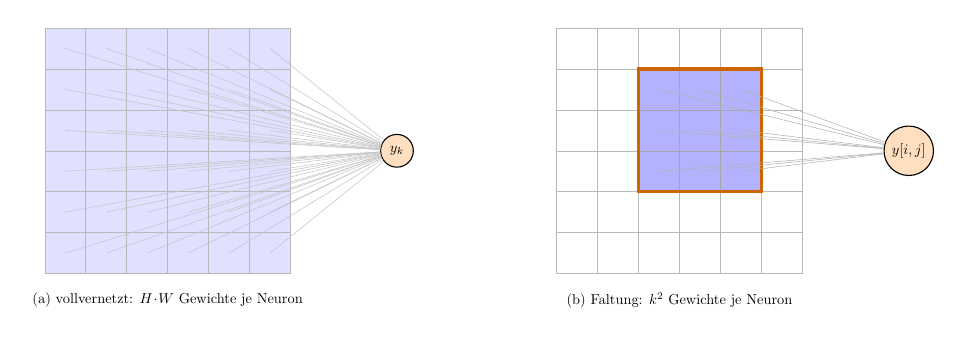
\begin{tikzpicture}[scale=0.52, every node/.style={transform shape}]
  % ---- Panel a: vollvernetzt ----
  \begin{scope}[shift={(0,0)}]
    \foreach \i in {0,...,5}{\foreach \j in {0,...,5}{
      \fill[blue!12] (\i,\j) rectangle ++(1,1);
      \draw[gray!55,very thin] (\i,\j) rectangle ++(1,1);}}
    \node (outa) at (8.6,3) [circle,draw,fill=orange!25,minimum size=8mm] {$y_k$};
    \foreach \i in {0,...,5}{\foreach \j in {0,...,5}{
      \draw[gray!45,very thin] (\i+0.5,\j+0.5) -- (outa);}}
    \node[below] at (3,-0.35) {(a) vollvernetzt: $H\!\cdot\!W$ Gewichte je Neuron};
  \end{scope}
  % ---- Panel b: Faltung ----
  \begin{scope}[shift={(12.5,0)}]
    \foreach \i in {0,...,5}{\foreach \j in {0,...,5}{
      \draw[gray!55,very thin] (\i,\j) rectangle ++(1,1);}}
    \foreach \i in {2,3,4}{\foreach \j in {2,3,4}{
      \fill[blue!30] (\i,\j) rectangle ++(1,1);
      \draw[gray!70,very thin] (\i,\j) rectangle ++(1,1);}}
    \draw[very thick,orange!80!black] (2,2) rectangle (5,5);
    \node (outb) at (8.6,3) [circle,draw,fill=orange!25,minimum size=8mm] {$y[i,j]$};
    \foreach \i in {2,3,4}{\foreach \j in {2,3,4}{
      \draw[gray!60,very thin] (\i+0.5,\j+0.5) -- (outb);}}
    \node[below] at (3,-0.35) {(b) Faltung: $k^2$ Gewichte je Neuron};
  \end{scope}
\end{tikzpicture}
\caption[Vollvernetzte Schicht gegen Faltungsschicht]{Lokale rezeptive Felder.
(a)~In einer vollvernetzten Schicht ist jedes Ausgabeneuron mit allen
$H\cdot W$ Eingangspixeln verbunden. (b)~In einer Faltungsschicht nach
Gleichung~\eqref{eq:conv} beschränkt sich die Summation auf
eine $k\times k$-Nachbarschaft; für $k=3$ sinkt die Zahl der Verbindungen je
Ausgabeneuron bei $640\times640$ Eingabe von 409\,600 auf 9. Zugleich wird
derselbe Kernel an allen Positionen verwendet (Weight Sharing), sodass die
Parameterzahl der Schicht unabhängig von der Bildgröße wird.}
\label{abb:rezeptivesfeld}
\end{figure}

Das theoretische rezeptive Feld wächst mit der Netztiefe. Bezeichnet $r_\ell$
seine Kantenlänge nach Schicht $\ell$, $k_\ell$ die Kernelgröße und $s_m$ die
Schrittweite der Schicht $m$, so gilt
\begin{equation}
r_\ell = r_{\ell-1} + (k_\ell - 1)\prod_{m=1}^{\ell-1} s_m,
\qquad r_0 = 1.
\label{eq:rf}
\end{equation}

Bei reinen $3\times3$-Faltungen mit $s_m = 1$ wächst $r_\ell$ nur linear; erst
Schrittweiten $s_m = 2$ lassen das Produkt exponentiell wachsen, sodass das
rezeptive Feld schnell große Bildbereiche umfasst. Daraus entsteht die
Merkmalshierarchie aus Abschnitt~\ref{sec:hierarchie}. Das \emph{effektive}
rezeptive Feld fällt dabei kleiner aus als dieses theoretische Maß:
\textcite{luo2016} zeigen, dass der Einfluss
$\partial y_{\text{Zentrum}} / \partial x[i,j]$ annähernd gaußförmig zum Zentrum
hin abfällt.

\absatz{Geteilte Gewichte (Weight Sharing).} Derselbe Kernel wird an allen
Positionen verwendet, formal $w_{ij} = w$ für alle $(i,j)$. Eine Schicht mit
$C_{\text{in}}$ Eingangs- und $C_{\text{out}}$ Ausgangskanälen hat dadurch
$C_{\text{out}} \cdot C_{\text{in}} \cdot k^2 + C_{\text{out}}$ Parameter --
\emph{unabhängig von der Bildgröße}, im Unterschied zur vollvernetzten Schicht.
Ein Muster, das nur an wenigen Positionen in den Trainingsdaten vorkommt, wird
damit überall erkannt.

Die zentrale Eigenschaft ist die \textbf{Translationsäquivarianz}. Bezeichnet
$(T_\tau x)[i,j] = x[i-\tau_1,\,j-\tau_2]$ die Verschiebung um $\tau$, so gilt
für die Faltungsoperation $f$:
\begin{equation}
f(T_\tau x) = T_\tau f(x).
\label{eq:aequivarianz}
\end{equation}

Eine Verschiebung der Eingabe führt also zu einer identischen Verschiebung der
Ausgabe. Gerechtfertigt ist das durch die näherungsweise Stationarität
natürlicher Bildstatistik -- eine Kante bleibt eine Kante, unabhängig von ihrer
Position \parencite{lecun1998,goodfellow2016}. Zu betonen ist, dass Äquivarianz
\emph{nicht} Invarianz bedeutet; diese entsteht erst durch das Subsampling.

\absatz{Räumliches Subsampling.} Für die Objekterkennung ist Invarianz gegenüber
kleinen Verschiebungen erwünscht, also $f(T_\tau x) \approx f(x)$ für kleine
$\|\tau\|$. Sie entsteht durch stufenweise Reduktion der räumlichen Auflösung --
klassisch durch Max-Pooling, in modernen Architekturen wie YOLO26 überwiegend
durch Faltungen mit Schrittweite $s = 2$. Erhalten bleibt dabei nur, \emph{ob}
ein Merkmal im Fenster auftrat, nicht seine exakte Position
\parencite{lecun1998,goodfellow2016}. Nach $L$ solchen Stufen beträgt die
Gesamtschrittweite $S = \prod_\ell s_\ell = 2^L$; die Zahl der räumlichen
Positionen sinkt um den Faktor $S^2$, was den mit der Tiefe wachsenden
Kanalzahlen entgegenwirkt.

Der Preis ist ein Verlust an Ortsinformation, und der wird bei kleinen Objekten
kritisch. Eine Zelle der Merkmalsebene mit Gesamtschrittweite $S$ entspricht
einem Bildbereich von $S \times S$ Pixeln; ein Objekt mit Durchmesser $d$ belegt
dort nur $d/S$ Zellen. Für $d < S$ ist es kleiner als eine einzelne Zelle und
strukturell nicht mehr zuverlässig lokalisierbar. Für die feinste
Standard-Detektionsebene P3 in YOLO26 gilt $S = 8$ -- ein Rohrprofil mit
$d = 6$ Pixeln unterschreitet diese Grenze. Dieser Zusammenhang begründet die
Multi-Skalen-Fusion moderner Detektoren (Abschnitt~\ref{sec:neck}) ebenso wie die
in Abschnitt~\ref{sec:anwendung} diskutierten Gegenmaßnahmen -- erhöhte
Eingabeauflösung und Kachelung --, die beide $d$ relativ zu $S$ vergrößern.

\absatz{Zusammenspiel.} Die drei Prinzipien greifen aufeinander auf: Lokale
rezeptive Felder senken die Verbindungen je Neuron von $H \cdot W$ auf $k^2$,
Weight Sharing löst die Parameterzahl von der Bildgröße, Subsampling reduziert
die Positionen um $S^2$ und erzeugt lokale Translationsinvarianz. Gemeinsam
kodieren sie die Annahmen, die für Bilddaten zutreffen -- Lokalität,
Stationarität und Toleranz gegenüber kleinen Verschiebungen
\parencite{lecun1998}.

\subsection{Merkmalshierarchie und Objektdetektion}
\label{sec:hierarchie}

Auf jede Faltung folgt eine nichtlineare Aktivierung -- heute überwiegend die
Rectified Linear Unit $f(x) = \max(0,x)$ oder Varianten wie SiLU
\parencite{krizhevsky2012} --, ohne die das Netz nur lineare Abbildungen lernen
könnte. Aus der Stapelung entsteht ein hierarchischer Aufbau der
Repräsentationen: Frühe Schichten reagieren auf Kanten und Farbverläufe, mittlere
auf Texturen und Teilstrukturen, tiefe auf semantische Objektbestandteile
\parencite{zeiler2014}. Diese datengetriebene Merkmalsextraktion tritt an die
Stelle des manuell entworfenen Feature Engineering und gilt als wesentlicher
Grund für die Leistungssprünge tiefer Netze \parencite{lecun2015}. Am Ende
klassischer Architekturen fassen vollvernetzte Schichten die Merkmale zusammen;
in modernen Detektoren sind sie vollständig durch Faltungen ersetzt
(Abschnitt~\ref{sec:neck}). Residualverbindungen \parencite{he2016} ermöglichen
das stabile Training sehr tiefer Netze und sind Standardbaustein nahezu aller
CNN-Backbones.

Für diese Arbeit ist nicht die Klassifikation relevant, sondern die
\textbf{Objektdetektion}: das gleichzeitige Lokalisieren und Klassifizieren
mehrerer Objekte. Zweistufige Detektoren erzeugen zunächst Regionsvorschläge und
klassifizieren diese anschließend \parencite{ren2015}; einstufige Detektoren
formulieren die Detektion als einmaliges Regressionsproblem und sagen in einem
Durchlauf direkt Boxen und Klassenwahrscheinlichkeiten vorher
\parencite{redmon2016,liu2016ssd}, was Echtzeitfähigkeit bei geringen
Genauigkeitseinbußen ermöglicht. Klassisch nachgeschaltet ist die
Non-Maximum Suppression (NMS), die redundante überlappende Detektionen anhand
ihrer Intersection over Union unterdrückt -- bei dicht gepackten gleichartigen
Objekten eine potenzielle Fehlerquelle.

\section{YOLO26}
\label{sec:yolo26}

\subsection{Einordnung und Neuerungen}

\enquote{You Only Look Once} wurde 2016 als erster echtzeitfähiger einstufiger
Detektor vorgestellt \parencite{redmon2016}; ab YOLOv8 übernahm Ultralytics die
Weiterentwicklung und etablierte ankerfreie, entkoppelte Detektionsköpfe
\parencite{sapkota2025}. YOLO26 wurde im September 2025 vorgestellt und
unterscheidet sich von YOLO11 durch vier koordinierte Änderungen: ein
Dual-Head-Design für NMS-freie Inferenz, den Wegfall der Distribution Focal Loss,
ProgLoss zusammen mit STAL sowie den MuSGD-Optimierer
\parencite{ultralytics2026,sapkota2025}.

Für diese Arbeit ist davon eine Änderung einschlägig: Die
\emph{Small-Target-Aware Label Assignment} garantiert positive Labelzuweisungen
auch für sehr kleine Objekte -- genau das Problem klassischer
Zuweisungsstrategien, das Abschnitt~\ref{sec:ioukleinobjekt} quantifiziert.

\subsection{Backbone, Neck, Head und die Merkmalspyramide}
\label{sec:neck}

YOLO26 folgt der Dreiteilung \textbf{Backbone $\to$ Neck $\to$ Head}. Das
Backbone reduziert die räumliche Auflösung stufenweise per Stride-2-Faltungen
($1024 \to 512 \to 256 \to 128 \to 64 \to 32$ bei $1024$\px{} Eingabe), während
die Kanalzahl wächst -- räumliche Präzision wird gegen semantische Tiefe
getauscht.

\absatz{Neck.} Das Neck verbindet die Auflösungsstufen in beide Richtungen
(FPN/PAN-Prinzip, \cite{lin2017fpn}): Tiefe, semantisch reiche Merkmalskarten
werden hochskaliert und mit den feinen, ortsgenauen Karten früherer Stufen
zusammengeführt, und umgekehrt. Der Head erhält dadurch mehrere Ausgabeebenen,
die nach Objektgröße zuständig sind. Die Standardkonfiguration liefert drei
Ebenen P3/P4/P5 mit den Gesamtschrittweiten 8/16/32; zusätzlich existiert eine
Konfiguration mit einer vierten, feineren Ebene \textbf{P2 mit Schrittweite~4}
(Abbildung~\ref{abb:pyramide}) -- eine Möglichkeit, die Auflösungsgrenze aus
Abschnitt~\ref{sec:ioukleinobjekt} nach unten zu verschieben, die in dieser
Arbeit aber nicht weiterverfolgt wird.

\begin{figure}[htbp]
\centering
\begin{tikzpicture}[x=1cm,y=1cm]
  % ---- Merkmalsebenen als Quadrate, Seitenlaenge proportional zur Gittergroesse
  \draw[fill=red!8,dashed,thick,red!60!black] (0,0) rectangle (4,4);
  \draw[step=0.5,gray!35,very thin] (0,0) grid (4,4);
  \draw[fill=blue!8] (4.7,0) rectangle (6.7,2);
  \draw[step=0.5,gray!35,very thin] (4.7,0) grid (6.7,2);
  \draw[fill=blue!8] (7.4,0) rectangle (8.4,1);
  \draw[step=0.5,gray!35,very thin] (7.4,0) grid (8.4,1);
  \draw[fill=blue!8] (9.1,0) rectangle (9.6,0.5);

  \node[below,align=center,font=\scriptsize] at (2,-0.2)
       {\textbf{P2} $\;$ Stride 4\\$256\times256$\\65\,536 Positionen};
  \node[below,align=center,font=\scriptsize] at (5.7,-0.2)
       {\textbf{P3} $\;$ Stride 8\\$128\times128$\\16\,384};
  \node[below,align=center,font=\scriptsize] at (7.9,-0.2)
       {\textbf{P4} $\;$ 16\\$64^2$\\4\,096};
  \node[below,align=center,font=\scriptsize] at (9.35,-0.2)
       {\textbf{P5} $\;$ 32\\$32^2$\\1\,024};

  \node[above,font=\scriptsize,red!60!black,align=center] at (2,4.15)
       {\emph{nur in der Variante} \code{-p2}};
  \node[above,font=\scriptsize,align=center] at (7.0,4.15)
       {Standardkonfiguration P3--P5};
  \draw[decorate,decoration={brace,amplitude=4pt},gray!60!black]
       (4.7,4.05) -- (9.6,4.05);
  \node[font=\scriptsize,align=left,anchor=west] at (10.1,2.6)
       {kleine\\Objekte};
  \node[font=\scriptsize,align=left,anchor=west] at (10.1,1.2)
       {große\\Objekte};
  \draw[-{Latex[length=1.6mm]},gray!60!black] (10.35,2.3) -- (10.35,1.6);
\end{tikzpicture}
\caption[Merkmalsebenen des Detektionskopfes]{Merkmalsebenen des
Detektionskopfes bei einer Eingabe von $1024\times1024$ Pixeln. Die
Seitenlänge der Quadrate ist proportional zur Gittergröße. Jede Zelle einer
Ebene mit Schrittweite $S$ entspricht einem Bildbereich von $S \times S$ Pixeln
und sagt Boxkoordinaten sowie Klassen-Scores vorher. Die Standardkonfiguration
nutzt \textbf{P3--P5}; die hier trainierten Modelle verwenden genau diese drei
Ebenen. Die links gestrichelt eingezeichnete Ebene P2 mit Schrittweite~4 gehört
zu einer Variante, die in dieser Arbeit nicht untersucht wird -- sie ist
mitabgebildet, weil sie zeigt, wie stark die Zahl der Prädiktionspositionen von
der Schrittweite abhängt: P2 allein enthält mehr Positionen als P3, P4 und P5
zusammen. Genau diese Abhängigkeit macht Abschnitt~\ref{sec:ioukleinobjekt} zum
Kern des Auflösungsproblems.}
\label{abb:pyramide}
\end{figure}

\absatz{Head.} Der Kopf ist vollständig faltungsbasiert: kleine
Faltungsstapel, die in $1\times1$-Faltungen münden. Eine $1\times1$-Faltung ist
äquivalent zu einer vollvernetzten Schicht über die Kanaldimension, wird aber
\textbf{positionsgeteilt} angewendet -- dieselbe Operation verarbeitet die Kanäle
jeder Gitterzelle separat. Das erhält die Translationsäquivarianz bis in die
Ausgabeschicht und macht das Netz unabhängig von einer festen Eingabegröße. Der
Kopf ist zusätzlich
\emph{entkoppelt} (getrennte Zweige für Klassifikation und Boxregression) und
\emph{ankerfrei}: Jede Gitterzelle regressiert direkt die Abstände zu den vier
Boxrändern. Damit ist die Zahl der Gitterzellen -- und nicht die Zahl der
Ankerboxen -- die Größe, die bestimmt, wie fein Objekte überhaupt aufgelöst
werden können.

\section{Anwendung auf gestapelte Bauzaunprofile}
\label{sec:anwendung}

Ein YOLO-Modell wird per Transfer Learning von COCO-vortrainierten Gewichten
\parencite{yosinski2014} auf eine einzige Objektklasse feinabgestimmt. Die
hierarchische Merkmalsextraktion des Backbones ist dafür gut geeignet:
Kreisförmige Metallprofile mit charakteristischem Hell-Dunkel-Verlauf sind
visuell einfache, texturarme Objekte, die bereits mittlere Netzschichten
repräsentieren können. YOLO26 adressiert die kritischen Eigenschaften des
Problems konzeptionell direkt: STAL und ProgLoss verbessern die Erkennung kleiner
Objekte, und die NMS-freie Inferenz eliminiert einen bei dicht gepackten
gleichartigen Objekten systematisch fehleranfälligen Hyperparameter -- ein zu
niedriger IoU-Schwellwert unterdrückt korrekte Detektionen benachbarter Rohre,
ein zu hoher lässt Duplikate zu. Da es sich um ein Ein-Klassen-Problem mit
geometrisch einfachen Objekten handelt, genügen kleine Modellvarianten.

Drei Grenzen sind kritisch. Erstens die \textbf{Auflösung}: Die
Standard-Eingabegröße von $640\times640$ ist für diese Aufgabe zu klein -- wird
eine hochaufgelöste Stapelaufnahme darauf herunterskaliert, schrumpfen die
Profile auf wenige Pixel und unterschreiten die Auflösungsgrenze der P3-Ebene.
Abhilfe schaffen eine erhöhte Eingabeauflösung (Rechenaufwand wächst
quadratisch), eine Kachelung des Bildes \parencite{akyon2022sahi} oder ein
feinerer Detektionskopf. Zweitens die
\textbf{Verdeckung}: Verkippte Zäune verdecken benachbarte Profile, und visuell
ähnliche Strukturen -- Gitterknoten, Löcher im Maschendraht, Schattenspalten --
drohen als Falschpositive. Drittens der \textbf{Datenbedarf}: Ein eigener
annotierter Datensatz ist unumgänglich und muss die reale Varianz abdecken. Genau
hier setzt der Praxisteil an -- die Domänenlücke wird nicht durch Handannotation
geschlossen, sondern durch eine Synthese-Pipeline, deren Entwurf Gegenstand der
Kapitel~\ref{kap:augtheorie} bis \ref{kap:trainingszeit} ist.
